\documentclass{article}
\usepackage{amsmath, amssymb, algpseudocode, graphicx}
\usepackage[margin=0.5in]{geometry}

\graphicspath{{images/}}

\DeclareMathOperator*{\argmin}{arg\,min}

\begin{document}

\title{Non-parametric Methods}
\author{Piyush Patil}
\maketitle

Most the other methods we've studied have been based on parameterized families of probability distributions, which formed the core of all the models we've used. We now turn to a form of statistics which makes no assumptions about the underlying probability distributions of any variables of objective functions in question. Non-parametric models still have parameters, of course, but are determined by the training data during training and adapted over time, rather considered a fixed set of quantities that describe an existing, immutable, ideal model which we wish to approximate.

\section{Kernel Trick}
Recall linear classifiers defined by separating hyperplanes, better known as SVMs (support vector machines), which, while using a linear function to classify data, could learn linearly inseparable data by lifting it to higher dimensions. A problem with this approach is that, even generalizing the polynomial regression with a degree $ p $ polynomial and feature vectors in $ \mathbb{R}^d $, there are $ O(d^p) $ possible features. This is more generally known as the \textit{curse of dimensionality}, and refers to the exponential nature of the increase of the volume of a search space with the number of dimensions, making many low-dimensional models intractable in higher dimensions.
\newline
With regard to SVMs, we can use the \textit{kernel trick} to lift feature vectors to implicit high dimensional space but without ever needing to compute the coordinates of the data in that space, thereby bypassing the curse of dimensionality. This is possible because in some cases, detailed below, we can find a function corresponding to the feature transformation which we can use to cheaply compute all the inner products of every pair of data points' images in high-dimensional space, which is often much cheaper than explicitly computing the coordinates, which is exponential in the number of coordinates (i.e. the number of dimensions).
\newline \newline
More generally, suppose we're given a dataset $ \{ (x_i, y_i), 1 \leq i \leq n \} $ for $ x_i \in \mathbb{R}^d $. It's often the case that we want to transform our data (e.g. lifting it to a higher dimensional space); let's represent this by passing each data point through the appropriate transformation function $ \phi: \mathbb{R}^d \rightarrow \mathbb{R}^p $, often called a \textit{feature map}. Note that in performing this transformation, although the dimensionality has increased, the total amount of information contained in the feature vectors is effectively the same; our hope is merely to change the shape of the data in space, to make it more amenable to simple machine learning models like linear classifiers. In other words, applying an SVM to the original dataset of $ (x_i, y_i) $ might not work since the data is not linearly separable, but applying it to $ (\phi(x_i), y_i) $ might. What's really happening here is we're looking for an appropriate $ \phi $ which exploits some internal, latent structure of the data and makes the structure more apparent, by using it to embed the data points in a higher-dimensional manifold in the hopes that the new representation is linearly separable. The problem is this poses another instance of the curse of dimensionality - even when $ p $ is only modestly larger than $ d $, it becomes very computationally expensive to both compute the $ \phi(x_i) $'s for every $ i $ and to perform operations with the $ \phi(x_i) $'s.
\newline \newline
The key insight in the \textit{kernel trick} is that because most mathematical operations necessary in applying machine learning models can be expressed in terms of inner products if we can find a function $ k $ such that $ k(x_i, x_j) = \langle \phi(x_i), \phi(x_j) \rangle $ then we can perform the necessary computations for our model, even in $ p $-dimensional space, without ever computing $ \phi $ at all, if we can reduce the model to inner products (where $ \langle \cdot, \cdot \rangle $ denotes some inner product); in fact, it no longer matters how large $ p $ is or if it's even finite, since computing $ k $, which is often computationally easy, doesn't depend on $ p $. Furthermore, such a $ k: \mathbb{R}^d \times \mathbb{R}^d \rightarrow \mathbb{R} $ is, under certain conditions, guaranteed to exist if we choose our transformation correctly. To see why, we begin by introducing some preliminary mathematical concepts in operator theory and functional analysis.
\newline \newline
\textbf{(Definition) Positive-Definite Kernel}: \textit{A symmetric function $ k: X \times X \rightarrow \mathbb{R} $, for some non-empty set $ X $, is \textbf{positive-definite} if}
$$ \forall f: X \rightarrow \mathbb{R}: \sum_{i = 1}^n \sum_{j = 1}^n f(x_i) k(x_i, x_j) f(x_j) > 0 $$
\indent \textit{holds for any $ n $ and elements $ x_i, x_j \in X $. When $ X $ is uncountable, the definition generalizes to}
$$ \int \int_{X^2} f(x) k(x, y) f(y) dx \hspace{0.02in} dy > 0 $$
\indent \textit{If the above inequalities aren't strict, then we say $ k $ is \textbf{non-negative-definite}.}
\newline
\indent \textit{Intuition}: Basically, the above definition generalizes the matrix definition of positive-definiteness, which states that a symmetric matrix $ A $ is positive-definite if for any vector $ x $, $ x^\intercal A x \geq 0 $, to function spaces. $ f(x_i) $ and $ f(x_j) $ can be considered transposes in some sense, if we consider the $ i $ index as running in one direction and the $ j $ index as running in another, orthogonal direction. This can be seen more clearly be rewriting the definition of matrix positive-definiteness as: a symmetric $ n \times n $ matrix $ A $ being positive-definite if
$$ x^\intercal A x = \sum_{i = 1}^n \sum_{j = 1}^n x_i A_{i, j} y_j \geq 0 $$
As with positive-definite matrices, positive-definite kernels have positive eigenvalues (where eigenvalues are defined as $ \lambda $ s.t. $ T_k(f) = \lambda f $; $ T_k $ is defined below), and their unit eigenfunctions (eigenfunctions associated with particular eigenvalues, with unit norm) are pairwise orthonormal.
\newline
\indent The motivation for kernels is that they're meant to be functions which act as weights for integral operators in operator theory, i.e. we define an integral operator $ T_k $ for kernel $ k $ which maps functions $ f $ to functions with $ T_k(f) = \int k(x, t) f(t) dt = (T_k f)(x) $, which is a kind of weighted average of the function which maps the function to another function, which, if we chose our kernel right, is easier to work with. Positive-definite kernels, specifically, can be viewed as similarity functions (functions which quantify to some degree how similar its two inputs are), in the sense that negative-definite kernels are analogous to distance functions. This is because whenever a negative-definite kernel uniquely vanishes on the set $ \{ (x, x), x \in X \} $ (so the it vanishes only at identical points), the function satisfies the positive-definiteness condition of a metric space, and so the square root of the kernel is a valid distance metric (as defined in the theory of metric spaces).
\newline
\indent \textit{Intuition for positive-definite matrices}: Positive-definite matrices have the unique property that they map vectors to vectors which are always within an angle of $ \frac{\pi}{2} $ from the input vector. This is analogous to what positive numbers do under multiplication - they scale numbers but never reflect about the origin in a complete reversal or directionality. We can intuitively think of positive-definite matrices as simply analogous multidimensional positive scalars. 
\newline \newline
Now that we have a definition of what kernels are, we can investigate possible uses for them in machine learning. When we build machine learning models we're working with feature vectors, not kernels, and the above definitions don't provide a way to, given feature vectors and a feature map, find a kernel that allows us to avoid actually computing the feature map. To proceed from here, we appeal to a powerful theorem in functional analysis, which essentially states that every kernel function, under certain conditions, can be expressed as a dot product in some feature space.
\newline \newline
\textbf{(Theorem) Mercer's Theorem}: \textit{Let $ k $ be a continuous, symmetric, non-negative-definite kernel. Let $ T_k $ be the integral operator associated with $ k $, and $ \{ e_i \}, \{ \lambda_i \} $ be the (orthonormal since $ k $ is non-negative definite, and hence an orthonormal basis) eigenfunctions and eigenvalues, respectively of $ T_k $. Then the $ e_i $'s are continuous, and we can represent $ k $ as}
$$ k(x, y) = \sum_{i = 1}^\infty \lambda_i e_i(x) e_j(y) $$
\indent \textit{Moreover, the above infinite series of functions converge absolutely and uniformly.
}\newline
This condition, for $ k $ to be continuous, symmetric, and non-negative-definite, is called \textbf{Mercer's condition}.
\newline
\indent \textit{Intuition}: First, to better understand the above theorem (which we won't prove here) we draw an analogy with properties of positive-definite matrices, as we did in the explanation of positive-definite kernels. The above theorem is analogous to the \textit{spectral theorem}. Recall that the spectral theorem, also known as \textit{symmetric eigenvalue decomposition}, is equivalent to the statement that any positive-definite $ n \times n $ matrix $ A $ can be written
$$ A = \sum_{i = 1}^n \lambda_i u_i u_i^\intercal = U \Lambda U^\intercal $$
where $ u_i, \lambda_i $ are the eigenvectors and eigenvalues, respectively, of $ A $, and $ U = \begin{bmatrix} u_1 \cdots y_n \end{bmatrix}, \Lambda = \text{diag}(\lambda_1, \cdots, \lambda_n) $. In other words, there exists an orthonormal basis such that $ A $ is diagonal in that basis. Mercer's theorem above makes almost the exact same statement, except with eigenfunctions instead of eigenvectors and with different arguments instead of transpose. So, we can interpret Mercer's theorem as the functional analytic extension of the spectral theorem from linear algebra, and essentially stating that kernels satisfying Mercer's condition are similarly "diagonal" in some orthonormal basis.
\newline \newline
Let's now explain the connection between Mercer's theorem and the kernel trick; to do this, we'll show that given that kernel $ k $ satisfies Mercer's condition, we can find a feature map over our input space $ \phi $, as described above, so that $ k $ represents the inner product of the feature transforms of input vectors. If our machine learning model only uses inner products of $ \phi(x_i) $ and not the $ \phi(x_i) $ itself, then we can replace every (expensive to compute) inner product of feature transforms with our kernel, thereby making it computationally feasible to perform feature lifting without dealing with the curse of dimenionality.
\newline
Recall that our function $ k $ mapped 2-tuples in $ X $ to real numbers; if $ X $ is finite, or even countably infinite, as it will be in any machine learning applications, then, letting $ X = \{ x_1, \cdots, x_n \} $ (i.e. we choose a kernel function whose domain is our input space), for input vectors $ x_i $, we can define the \textit{kernel matrix}, or \textit{Gram matrix}, $ K $ by
$$ K_{i, j} = k(x_i, x_j) $$
It follows that $ K $ is symmetric, and so by the spectral theorem we can decompose
$$ K = V \Lambda V^\intercal $$
where $ V $'s columns are the eigenvectors of $ K $ and $ \Lambda = \text{diag}(\lambda_1, \cdots, \lambda_m) $ for eigenvalues $ \lambda_i $ of $ k $. We're now in a position to explicitly define the feature map we alluded to above: define $ \phi $ over our input space $ X $ by
$$ (\phi(x_i))_j = \sqrt{\lambda_j} (v_j)_i = \sqrt{\Lambda_{j, j}} V_{i, j} $$
Then we can write the inner product of feature transformations of our input vectors in terms of $ k $ as follows.
$$ \langle \phi(x_i), \phi(x_j) \rangle = \sum_{t = 1}^m \lambda_t (v_t)_i (v_t)_j = (V \Lambda V^\intercal)_{i, j} = K_{i, j} = k(x_i, x_j) $$
The reason we need Mercer's condition for the above to hold is that Mercer's condition implies that the eigenvalues of $ K $ are all positive, allowing us to avoid complex inner products (even when we're working over the complex numbers, negative eigenvalues have other issues we won't go into).
\newline \newline
We've thus shown that if we want to lift our input vectors to a higher dimension with some feature map, we just have to find an associated kernel which satisfies Mercer's condition, and we'll be able to by pass the computation of inner products of the feature maps entirely in favor of computing the kernel.

\subsection{Common Feature Maps and Associated Kernels}
Here are some of the most commonly used feature maps, and their associated kernels $ k $.
\newline
\begin{center}
    \begin{tabular}{c | c}
        \textit{Type} & $ k $ \\
        \hline
        Linear & $ k(x, y) = x^\intercal y + c $ \\
        Polynomial of degree $ p $ & $ k(x, y) = (x^\intercal y + c)^p $ \\
        Gaussian & $ k(x, y) = \exp \left(- \frac{| x - y |^2}{2 \sigma^2} \right) $ \\
        Exponential & $ k(x, y) = \exp(- \frac{1}{2} | x - y |) $ \\
        Sigmoid & $ k(x, y) = \tanh(x^\intercal y + c) $ \\
        Inverse multiquadratic & $ k(x, y) = \frac{1}{\sqrt{| x - y |^2 + c}} $
    \end{tabular}
\end{center}
where $ c \in \mathbb{R} $ above. Kernels satisfying Mercer's condition are often called \textit{Mercer kernels}. There are infinitely many Mercer kernels, and many more than the above listed used in practice; kernels are adapted for the problem at hand, and differ greatly in different applications, from computer vision to NLP, etc. We can build new Mercer kernels from old ones, as the space of such kernels is convex. Thus, for Mercer kernels $ k_1, k_2 $,
$$ a_1 k_1 + a_2 k_2, k_1 k_2 $$
are Mercer kernels as well (for real scalars $ a_1, a_2 $). Moreover, if $ f $ is a polynomial in one variable, $ f(k_1) $ is a Mercer kernel (this follows from the above), but we also have the more surprising result that $ \exp(k_1) $ is a Mercer kernel too (this can be proven by letting $ f $ be the truncated Taylor series for the exponential function and taking the limit). If $ g $ is a real-valued function then $ k(x, y) := g(x) g(y) $ is a Mercer kernel; more generally, $ k(x, y) = k_1(g(x), g(y)) $ is a Mercer kernel. Finally, if $ A $ is a positive-definite matrix, then $ k(x, y) = x^\intercal A y $ is a Mercer kernel.
\newline
In particular, let's look at the Gaussian kernel, one of the most common kernels used in practice.
\newline \newline
\textbf{Gaussian kernel}: Also known as the \textbf{radial basis function} (RBF) kernel, the Gaussian kernel is the function
$$ k(x, y) = \exp \left( - \frac{| x - y |^2}{2 \sigma^2} \right) $$
\indent and, in the one-dimensional case (which generalizes), is associated with the feature map
$$ \phi(x) = \exp \left( - \frac{x^2}{2 \sigma^2} \right) \begin{bmatrix} 1 & \cdots & \frac{x^j}{\sigma^2 \sqrt{j!}} & \cdots \end{bmatrix}^\intercal $$
\indent Notice that the feature representation is an infinite vector (though the dot product $ \phi(x)^\intercal \phi(y) $ exists and forms a convergent infinite series), and our regression function becomes a weighted sum of Gaussians with each Gaussian centered at a unique input vector. In practice, this gives a very smooth regression function.
\newline
Now that we've explained the theoretical underpinnings of kernel methods, we spend the next few sections exploring some example applications of the kernel trick to common models we've studied.

\subsection{Kernelized Ridge Regression}
Let's apply the above theory to ridge regression, as an example. Recall that ridge regression with a data matrix $ X \in \mathbb{R}^{n \times (d + 1)} $ (i.e. input vectors as rows) and label vector $ y \in \mathbb{R}^n $ has solution
$$ w = (X^\intercal + \lambda I)^{-1} X^{\intercal} y $$
where $ \lambda $ is the scaling factor for the regularization term. Note that in the exact solution we use $ I' $, not $ I $ (the identity matrix), which is the identity matrix with the bottom right entry set to zero, so as to avoid penalizing the translation term in $ w $. If we center $ X $ by mapping $ x_i $ to $ x_i - \mu $ for, where $ \mu $ is the mean of the dataset, then the expected value of $ w_{d + 1} $ (the translation term) is zero anyways, so we can ignore this technicality.
\newline
First, let's rewrite the ridge regression equations in terms of kernel functions. It turns out we can rewrite $ w $ as a linear combination of our sample points (it's quite an elegant yet almost expected result that the optimal parameter in linear regression is a linear combination of the data), if we make the following observations.
$$ (X^\intercal X + \lambda I) X^\intercal = X^\intercal X X^\intercal + \lambda X^\intercal = X^\intercal \cdot (X X^\intercal + \lambda I) $$
$$ \rightarrow (X^\intercal X + \lambda I)^{-1} (X^\intercal X + \lambda I) X^\intercal \cdot (X X^\intercal + \lambda I)^{-1} y = (X^\intercal X + \lambda I)^{-1} X^\intercal \cdot (X X^\intercal + \lambda I) \cdot (X X^\intercal + \lambda I)^{-1} y $$
$$ \rightarrow X^\intercal \cdot (X X^\intercal + \lambda I) y = (X^\intercal X + \lambda I)^{-1} X^\intercal y = w $$
$$ \rightarrow w = X^\intercal \alpha \text{ where } \alpha = (X X^\intercal + \lambda I)^{-1} y $$
Thus, our regression function becomes
$$ f(x) = w^\intercal x = \alpha^\intercal X x = \sum_{i = 1}^n \alpha_i \cdot (x^\intercal_i x) $$
Now, if we let our kernel function be $ k(v_1, v_2) = v_1^\intercal v_2 $, then the kernel matrix is $ K = X X^\intercal $ (so that, by definition, $ K_{i, j} = k(x_i, x_j) $), and we have
$$ f(x) = \sum_{i = 1}^n \alpha_i k(x_i, x) \text{ and } \alpha = (K + \lambda I)^{-1} y $$
\newline
Now that we've expressed the ridge regression equation in terms of a kernel function $ k $, let's see how we can use the kernel trick to circumvent the curse of dimensionality. The above equation demonstrates the power of the kernel trick - $ f(x) $ depends explicitly only on $ k $ and $ \alpha $, which in turn depends on $ K $; nowhere in the computation of $ f(x) $ is $ X $ explicitly used. If we wanted to apply some feature map $ \phi $ to our input vectors, in order to lift them to a higher dimensional space, normally we'd have to expensively construct $ \phi(X) $ by mapping each $ x_i $ to $ \phi(x_i) $, but with kernelization we could merely replace the kernel function $ k $ in the above equation with the kernel function associated with $ \phi $, call it $ k_{\phi} $, and moreover compute $ K_{i, j} = k_{\phi}(x_i, x_j) = \phi(x_i)^\intercal \phi(x_j) $ from $ \phi $'s kernel in order to compute $ \alpha $. We can avoid computing $ \phi(x_i) $ entirely, and compute $ k_\phi $ instead, a much cheaper operation. More fundamentally, the computation of $ k_\phi $ doesn't depend on the dimensionality of $ \phi $. We can therefore compute $ \phi(x_i)^\intercal \phi(x_j) $ in $ O(d) $ time, rather than $ O(d^p) $ time, even though $ \phi(\cdot) $ has length $ O(d^p) $, allowing us to lift features to arbitrarily high dimensions, even infinitely many, so long as we can compute the kernel of the feature map. One thing to note here - kernel methods are not always better than feature methods, since although the kernel doesn't depend on the dimensionality of the data, it does depend on the number of data points. Computing feature representations is more computationally efficient than computing the kernel if there are a relatively small number of features and a relatively large number of training samples.

\subsection{Kernelized Perceptrons}
Recall the original perceptron algorithm for a data matrix $ X $ and labels $ y $:
\begin{algorithmic}
    \Procedure{Perceptron}{}
        \While{$ \exists i \text{ s.t. } y_i x_i^\intercal w < 0 $}
            \State $ w \gets w + \eta y_i x_i $
        \EndWhile
    \EndProcedure
\end{algorithmic}
with predictor function $ f(x) = \text{sgn}(w^\intercal x) $. As with ridge regression, we can kernalize by using a linear combination of the input points by using a linear kernel. Let $ a $ be a vector such that $ w = X^\intercal \alpha $, so that $ x_i^\intercal w = (X X^\intercal \alpha)_i = (K \alpha)_i $ where $ K = X X^\intercal $ is our kernel matrix, defined as usual by $ K_{i, j} = k(x_i, x_j) = x_i^\intercal x_j $. After computing $ K $, we can run the following dual perceptron algorithm using the kernel:
\begin{algorithmic}
    \Procedure{DualPerceptron}{}
        \While{$ \exists i \text{ s.t. } y_i \cdot (K \alpha)_i < 0 $}
            \State $ \alpha_i \gets \alpha_i + \eta y_i $
        \EndWhile
    \EndProcedure
\end{algorithmic}
Once we've trained $ \alpha $, we can classify using
$$ f(x) = \text{sgn} \left( \sum_{i = 1}^n \alpha_i y_i k(x_i, x) \right) $$
as we designed. We can think of $ \alpha $ is a "mistake counter", keeping track of where our classifier had mis-classified and adjusting the weight of the corresponding input vector in our representation of $ w $ as a linear combination of input vectors. From a complexity perspective, the above algorithm isn't faster than the original perceptron algorithm, but if we wanted to apply a feature map $ \phi $ to the input vectors $ X $, we could avoid computing $ \phi(x_i) $ entirely, by replacing $ k $ in the above algorithm with $ \phi $'s kernel.

\subsection{Kernelized Logistic Regression}
Recall that in logistic regression, we use a cross-entropy error function
$$ J(w) = \sum_{i = 1}^n (y_i \log(s(x_i)) + (1 - y_i) \log(1 - s(x_i))) $$
where $ s $ is the logistic function,
$$ s(x) = \frac{1}{1 + \exp(- w^\intercal x)} $$
We computed the derivative of $ J $ with respect to $ w $ and used it in gradient descent to find the optimal $ w $. In the kernelized problem, we modify this algorithm in a very similar way to our modification of the perceptron algorithm. We again express $ w $ as a linear combination of our input vectors: $ w = X^\intercal \alpha $. Using a linear kernel and kernel matrix $ K = X X^\intercal \rightarrow K_{i, j} = k(x_i, x_j) = x_i^\intercal x_j $, we can perform gradient descent as before, but with the update equation
$$ \alpha_i \gets \alpha_i + \eta \cdot (y_i - s(K \alpha)_i) $$
Then, similar to before, we can compute our prediction of $ x $ by
$$ f(x) = s \left( \sum_{i = 1}^n \alpha_i k(x_i, x) \right) $$
As before, this allows us to pass $ X $ through a feature map $ \phi $ and replace the above equations with $ k_\phi $ instead of $ k $ to achieve the same results.

\section{Nearest Neighbors}
$ k $-nearest neighbors, often abbreviated kNN, is one of the most simplistic models in use. The key idea is simply to keep track of our dataset $ \{ (x_i, y_i), 1 \leq i \leq n \} $ so that when we're given a new data point we've never seen $ x $, we can approximate
$$ f(x) = f \left( \argmin_{x_i} d(x_i, x) \right) $$
for some distance metric $ d $, most commonly the Euclidean distance $ d(x, y) = | x - y |^2 $. In other words, we simply classify $ x $ into the class of the data point (from our dataset) closest to it. This is actually a special case with $ k = 1 $. To generalize rather than taking the class of the closest data point, we find the $ k $ nearest data points and have them "vote" on the class of $ x $, i.e. we choose the most common class among the $ k $ nearest data points to $ x $. If we're performing regression or have a continuous classification problem, we replace the vote with the average of the values of the $ k $ nearest data points. While the algorithm is extremely simple, it has the advantage of constant (in fact, $ O(0) $) training time.
\newline
We can visualize this with a Voronoi diagram. We're essentially partitioning the input space into disjoint subsets (each dependent on the $ k $ data points inside it) that are each associated with a class (the vote of the $ k $ data points in the subset); we classify new points merely by the class of the subset in which they fall.
\newline
One issue is that in high-dimensional space, computing the distance function for $ n $ points can be expensive.

\section{Decision Trees}
Decision trees are another simple, non-parametric model that can be used for both classification and regression. Their origins lie in classification problems, so we discuss these first. The idea is simple - we essentially test feature vectors against a set of boolean conditionals, and classify based on which attributes of the feature vector were true and which were false. We organize these boolean conditionals into a binary tree structure, so that the set of conditionals a feature vector is tested against depends on its answer to a prior conditional. Each node in the tree consists of a conditional, and the node's children represent recursive decision trees to test against, depending on the feature vector's answer to the node's conditional. We classify based on leaf nodes, either by associating leaf nodes with a class or by associating leaf nodes with a probability, say in binary classification. For regression, leaf nodes can also have real numbers representing our regression function, creating a piecewise constant regression function.

\begin{figure}[h]
    \center
    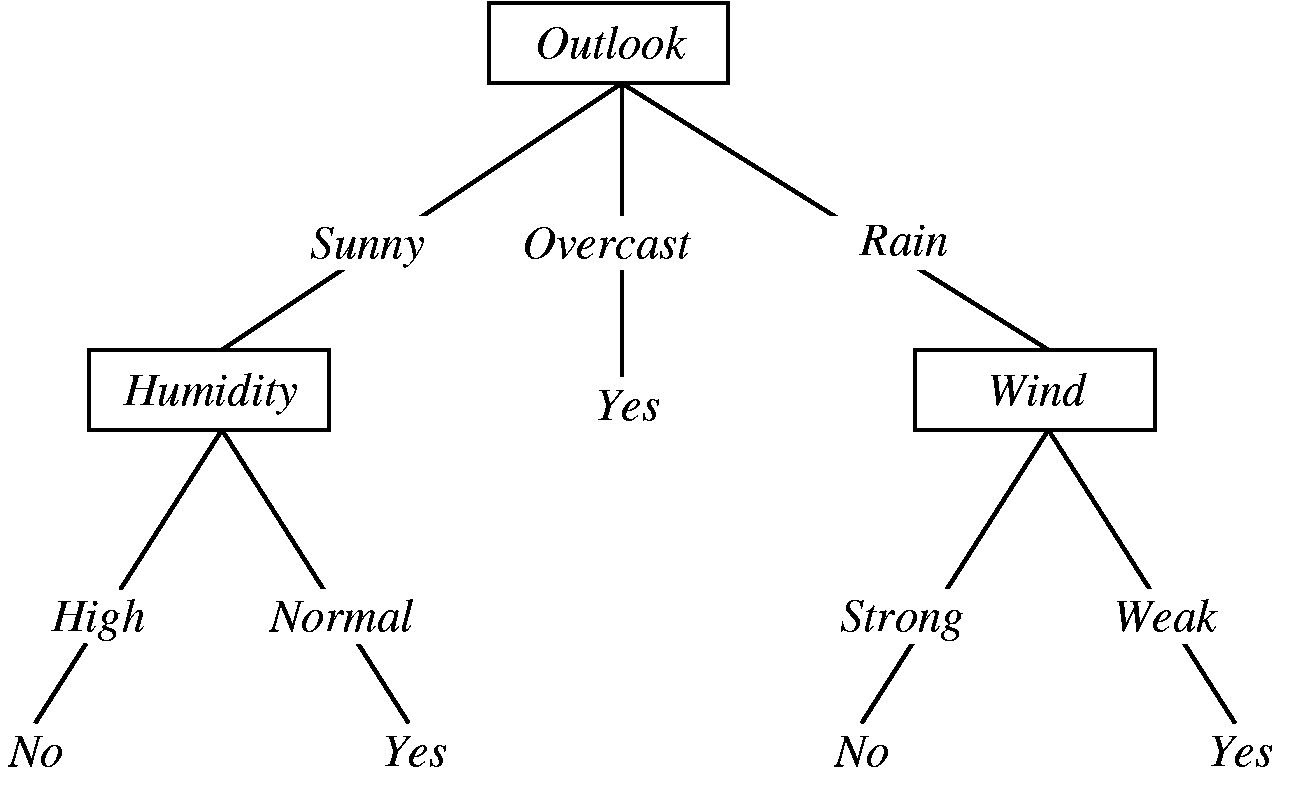
\includegraphics{decision_tree.png}
    \caption{Decision tree for if a given day is ideal for playing tennis.}
\end{figure}

As shown above, we can generalize beyond booleans to structure the tree according to several, not just two, answers to the conditionals at each node, in a general tree with an arbitrary number of children. Therefore, decision trees represent a recursive logical disjunction of conjunctions of constraints; every path from root to leaf represents a specific set of attributes met by the feature vector. Decision trees are therefore non-linear (in fact, non-continuous) methods for classification and regression. In fact, decision trees can be thought of as piecewise collections of disjoint linear classifiers, with the restriction that decision trees can only use hyperplanes parallel to a coordinate plane.

\subsection{Training}
The algorithm to train decision trees is, unsurprisingly, recrusive and quite simple. The idea is to simply find a good splitting point in our dataset, use it as the conditional for our root node, and recurse on the split dataset, stopping when no splitting point exists. This method can be generalized to an arbitrary number of splits at each node.

\begin{algorithmic}
    \Procedure{TrainBinaryDT}{$ D = \{ (x_i, y_i), 1 \leq i \leq n \} $}
        \If{every $ y_i $ is class $ C $}
            \State \textbf{return} leaf node with class $ C $
        \Else
            \State Choose the optimal splitting point, $ w \in \mathbb{R} $
            \State Partition the dataset into $ D_1 = \{ (x_i, y_i) \text { s.t. } (x_i)_j < \beta, \forall j \}, D_2 = \{ (x_i, y_i) \text { s.t. } (x_i)_j \geq \beta, \forall j \} $
            \State Create node $ N $  with $ w $
            \State Set left child of $ N $ to $ \textproc{TrainBinaryDT}(D_1) $, right child to $ \textproc{TrainBinaryDT}(D_2) $
            \State \textbf{return} $ N $
        \EndIf
    \EndProcedure
\end{algorithmic}
Of course, we haven't gone over how to find the optimal splitting point, or what optimal even means in this context. We can formalize this by introducing a loss function $ L $ on the data $ D $, and choose
$$ \argmin_{D_1, D_2} (L(D_1) + L(D_2)) \text{ where } D_2 = D - D_1 $$
Choosing a good loss function, however, can be tricky, since we want to maintain the property that the sum of the losses of $ D_1, D_2 $ should improve over the loss of $ D $ whenever our algorithm makes progress. One good cost function takes an idea from information theory - we measure the \textit{entropy} of the dataset. 
\newline \newline
\textbf{Entropy}: Here, we give a non-rigorous, intuitive introduction to \textit{Shannon entropy}, which we'll use in imposing a good loss function on your dataset for use in the decision tree training algorithm. For a random label $ y $ from our dataset, let's try to define some notion of \textit{surprise} that $ y = C $ for a class $ C $, where $ \text{Pr}(y = C) = 0 \rightarrow $ infinite surprise whereas $ \text{Pr}(y = C) = 1 \rightarrow $ zero surprise. We can expect $ y = C $ approximately once in every $ \text{Pr}(y = C)^{-1} $ events. The minimum amount of information it would require to fully describe $ \text{Pr}(y = C) $ is thus $ \log(\text{Pr}(y = C)^{-1}) $ bits. We therefore define the \textit{surprise} of the event $ y = C $ as $ - \log(\text{Pr}(y = C)) $, and define the \textit{Shannon entropy} as the of a set as the expected surprise:
$$ H(S) = - \sum_{C \in S} \text{Pr}(y = C) \log(\text{Pr}(y = C)) \text{ for random $ y $} $$
\indent The precise mathematical motivation for using the negative logarithm of the probability is simply that given that Shannon entropy is meant to serve as a measure of the expected information content of a random variable, we impose the following desirable conditions on the Shannon entropy:
\begin{enumerate}
    \item Decreases with probability: Rare events should have higher entropy than common ones.
    \item Non-negative: Entropy should never be negative.
    \item Events with probability 0 should have infinite entropy, while events with probability 1 should have zero entropy.
    \item Entropy should be additive for independent events.
\end{enumerate}
\indent The negative logarithm (or, equivalently, logarithm of the inverse) is the only function satisfying the above conditions.
\newline \newline
We can use Shannon entropy to quantify the intuitive notion that at each step of the training algorithm, we want to choose the most informative split over our data; we want to split the data so as to maximize \textit{information gain}, which, since entropy is a measure of surprise is the opposite of entropy. In other words, we want our decision tree to converge to lower entropy (i.e. higher certainty) in each leaf node, until the datasets represented by the leaves are completely pure and have zero entropy. After splitting, the weighted average entropy is
$$ H_{D_1, D_2} = \frac{|D_1| H(D_1) + |D_2| H(D_2)}{|D_1| + |D_2|} $$
We can now define our loss function as negative the information gain, or equivalently as the \textit{entropy gain}:
$$ L(D_1, D_2) = - (H(D) - H_{D_1, D_2}) = H_{D_1, D_2} - H(D) $$
We can therefore find the optimal loss function by iterating over all possible splits and choosing the one which minimizes $ L $. The resulting training algorithm has runtime $ O(n d h) $ where $ h $ is the depth or height of the decision tree; this is actually a reasonable runtime, since $ n d $ is the size of our data matrix $ X $ and $ h $ is typically logarithmic. Actually running the decision tree takes logarithmic time, $ O(\log(n)) $. Let's now explore some optimizations we can make.
\newline \newline
\textbf{Multivariate splits}: The above section on training focuses on the special case for split points with a single parameter $ w $, which is what restricted us to collections of separating hyperplanes that were parallel to a coordinate plane. If we generalize to multivariate splits, where for feature vector $ x $ the conditional at a node becomes $ w^\intercal x < \beta $ for vector $ w $ and scalar $ \beta $, our decision tree can now make use of collections of arbitrary hyperplanes, giving us all the power of SVMs, gaussian discriminant analysis, logistic regression, etc. but in a highly interpretable and simple model that also has the unique ability to hierarchically classify points, similar to kNN.
\newline \newline
\textbf{Stopping early}: In practice, running the decision tree training algorithm until all the leaves belong completely in a single class yields excessively deep trees that usually overfit. To combat this, we might stop the training algorithm prematurely. Some good stopping criteria are to stop when most of the points in a leaf (say, above 95\%) belong to the same class (this accounts for outliers), when the depth gets too large, when the information gain from additional splitting is too low, with cross-validation (this is especially effective), etc.
\newline \newline
\textbf{Pruning}: The idea here is simple - instead of stopping early, we build the full decision tree, which has most likely overfit the data, and fix the problem with the following greedy algorithm. Starting at leaves, we iteratively remove split points, merging leaves, until cross-validation accuracy stops improving. This often works better than stopping early because the information gained by splits is often erratic and unpredictable. It's often the case that a split that makes a lot of progress only follows after several mediocre splits. If we'd stopped early, we never would have discovered the optimal split.

\section{Random Forests and Ensembling}
Despite any optimizations we could make, decision trees tend to have very high variance, since they're so dependent on the format and order of the data. Nonetheless, they're still good models with low bias (we know they have the potential to be at least as powerful as SVMs, for example). In order to maintain the integrity of the model but lower the variance, we turn to \textit{ensemble learning}. The approach is simple - we simply train several decision trees and take the average (for regression) or majority by voting (for classification). Of course, this approach generalizes beyond decision trees, andewe often train several different models with different learning algorithms and average them to get a final ensemble learner, but the method works especially well for decision trees. The advantage to this is that some overfitting and resulting high variance for a particular model is okay, since we average our the variance in the end anyways. This means that an ensemble of deep decision trees is often better than a single decision tree.
\newline
When using the same model, one approach to ensure we have random starting points for each model, so as to reduce variance, is called \textit{bagging}, where we train each model on a random subsample of the data. The key idea is that when sampling for our subsamples, we sample with replacement.

\subsection{Random Forests}
One problem with ensembling on decision trees is that the resulting decision trees tend to turn our very similar, since if there's a particularly good split, they'll all discover it and proceed from there. TODO

\end{document}
